\section[Studies with the Hadron Outer Calorimeter]{Studies with the Hadron Outer Calorimeter \footnote{corresponding author: Yusuf Erdogan}}
\label{sec:HOstudies}
	In this section studies on detection efficiency of high energetic muons in the hadron outer calorimeter (HO) using 2012 data are shown.
	In addition the detection efficiency for cosmic muons from GRIN data is studied.
	\subsection{Studies on detection efficiency of prompt muons using 2012 data}
		Due to the similarity of the setup of HO and the proposed MTT we expect to find answers to some open questions concerning the MTT concept e.g. the muon detection capability of a
		scintillator system read out by SiPMs by studying the HO signals.
		In particular the detection efficiency for tight ID muons from Run A of the 2012 data in HO has been studied.
		The used dataset (/SingleMu/Run2012A-22Jan2013-v1/RECO) is from the re-reconstruction campaign January 2013.
		Thereby the SingleMu stream contains several HLT trigger paths each with at least one triggered muon with different conditions like a $p_T$ requirement or an isolation criterion.
		The muons from this dataset have to fulfill some selection criteria and also they have to be accepted by the HO system.
		The latter is necessary because of inefficient areas of HO caused for example by the supporting structures of CMS like the chimney \cite{JINST}.
		Before this selection can be done, the events have to fulfill some cleaning procedure.
		First of all the events from beam background are removed.
		Than a primary vertex filter is applied \cite{CMS-PAPER-TRK-11-001}:
		Using the vertex collection \verb+offlinePrimaryVertices+ only the events are chosen, in which vertices could be found whose:
			\begin{itemize}
				\item minimum number of degrees of freedom is 4,
				\item maximum distance on the $z$ axis to the origin of the coordinate system of CMS is 24\,cm,
				\item maximum impact parameter $d_0$ is 2\,cm.
			\end{itemize}
		\subsubsection{Muon selection and acceptance by HO}
		\label{thesectionhere}
			To ensure to have no misidentified muons going through the HO tiles selection criteria are set for the reconstructed muons:
			Only reconstructed global muons are chosen and their transverse momentum $p_T$ must be greater than 26\,GeV.
			Then a cut on the pseudorapidity of the muons, $|\eta_\mu| < 0.9$, is applied to ensure that they are in the barrel region and especially in the region of HO.
			Furthermore the muons have to have a tight ID.
			In \cite{CMS-PAPER-MUO-10-004} all requirements on muons to be a tight muon are given. \\
			Additionally all these selected tight muons should have a particle flow based combined relative isolation $I<0.2$ defined as
			\begin{equation}
				I = \frac{\sum{E_T^{chHad}} + \sum{E_T^{neutHad}} + \sum{E_T^\gamma}}{p_T}
			\end{equation}
			where $E_T^{chHad}$ is the transverse energy of a charged hadron in a cone of $\Delta R = 0.4$ around the muon, $E_T^{neutHad}$ same for a neutral hadron and $E_T^\gamma$ for a photon.
			Since the HO system does not cover the whole $\eta$-$\varphi$ plane - for example there are no tiles between the wheels - and since the HO system also has some areas with electronic inefficiencies
			the cut on $|\eta_{\mu}|$ mentioned before is not sufficient and a more sophisticated geometrical acceptance has to be required.
			This is done by using the \verb+MuonHOAcceptance+ class implemented in CMSSW.
			\verb+MuonHOAcceptance+ contains the entire HO geometry and allows boolean decisions on whether a muon is in the geometrical acceptance of the HO or not and also whether a muon is in the
			acceptance region of tiles that are working properly.
			It is also possible to accept or reject muons in regions with SiPM instrumented tiles (Fig.\ \ref{fig:ho_acceptance}). \\
			\begin{figure}[htbp]
				\centering
				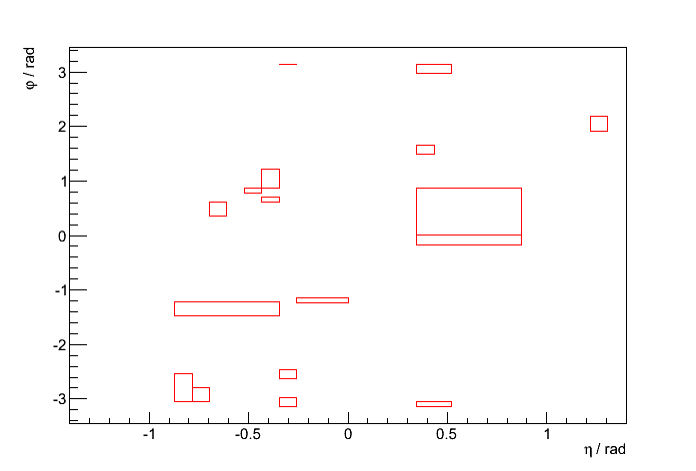
\includegraphics[width=0.45\textwidth]{Figures/erdogan/deadregions.png}
				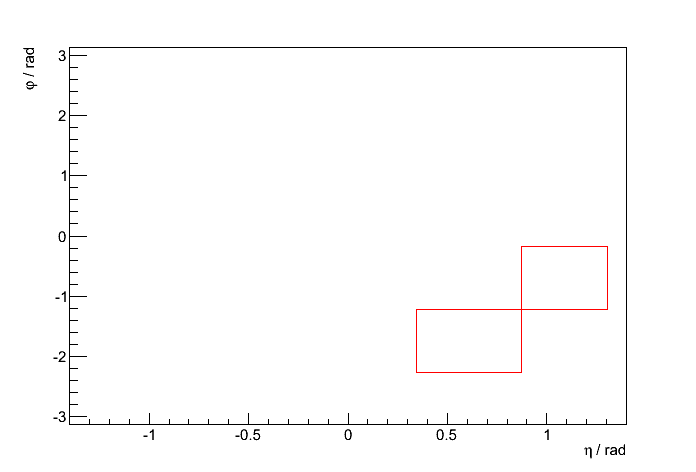
\includegraphics[width=0.45\textwidth]{Figures/erdogan/sipmregions.png}
				\caption{Left: In the $\eta$-$\varphi$ plane, the red rectangles are showing the regions, where HO is insensitive because of the supporting material or electrical issues (see also \cite{JINST}).
				Right: In red rectangles the acceptance regions for tiles with SiPM readout (status pre LS1) is depicted.}
				\label{fig:ho_acceptance}
			\end{figure}
			In Fig.\ \ref{fig:simhits_in_acceptance} the $\eta$-$\varphi$ distribution of simulated hits of muons with $p_T = 100$\,GeV (muon gun) in HO is shown.
			\begin{figure}[htbp]
				\centering
				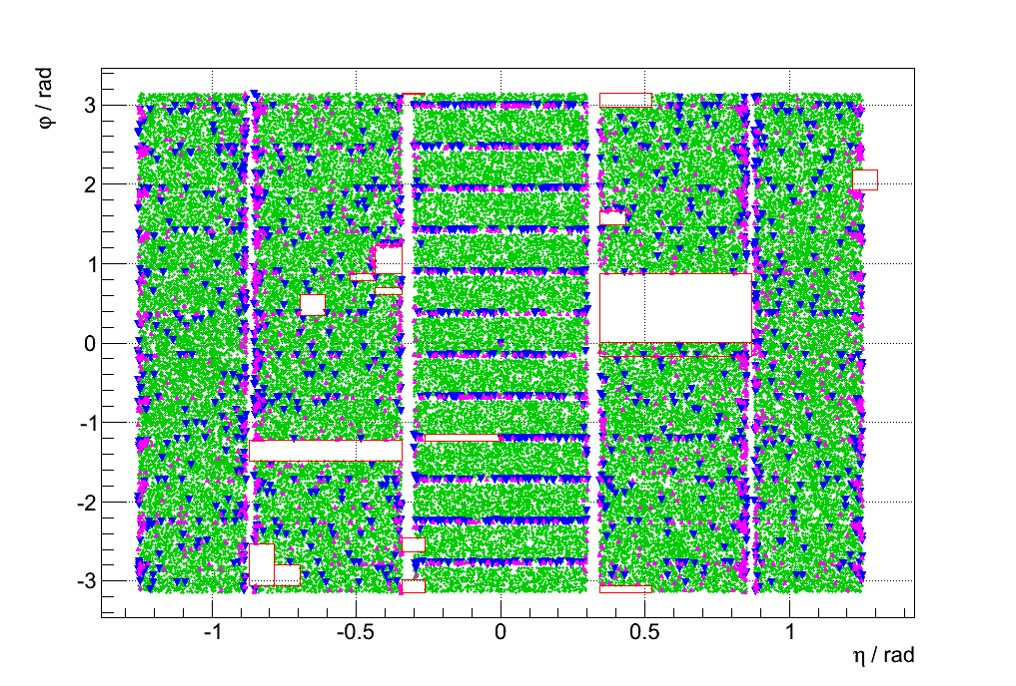
\includegraphics[width=0.45\textwidth]{Figures/erdogan/simhits_wo_deta_dphi.png}
				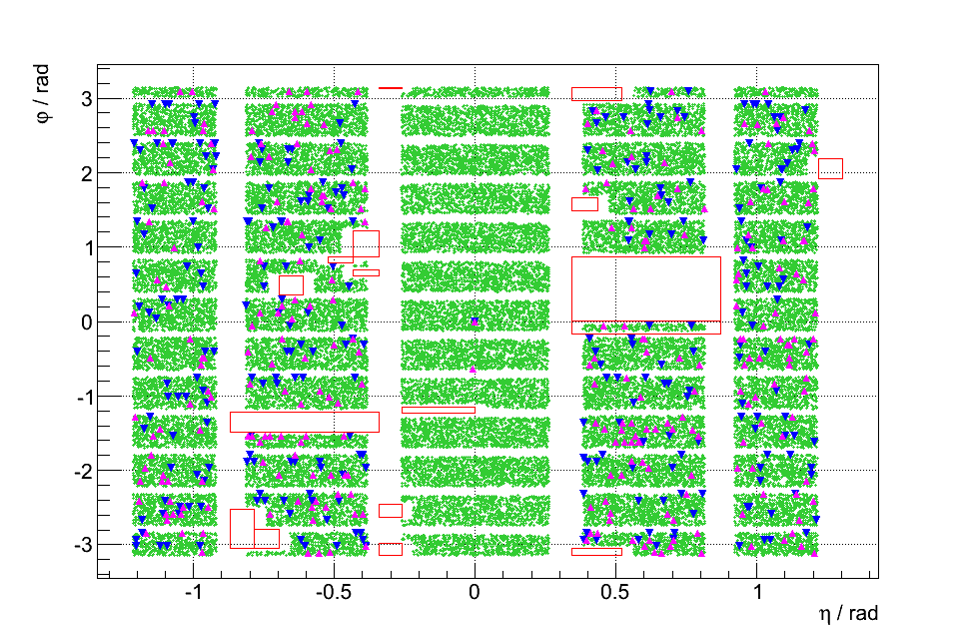
\includegraphics[width=0.45\textwidth]{Figures/erdogan/simhits_with_deta_dphi.png}
				\caption{Left: $\eta$-$\varphi$ distribution of simulated hits of muons with $p_T = 100$\,GeV (muon gun). In green, hits from geometrically accepted muons with energy depositions above 1.4\,MeV, in
				blue, same for muons with energy depositions between 0 and 1.4\,GeV and in magenta, for muons with no energy deposition at all. The threshold at 1.4\,MeV is motivated by the Bethe-Bloch formula,
				which predicts an energy deposition of larger than 1.4\,MeV for muons going through 1\,cm scintillator material. Right: The same distribution with the safety margins $d\eta = 0.04$ and
				$d\varphi = 0.017$ from the edges of the HO panels.}
				\label{fig:simhits_in_acceptance}
			\end{figure}
			According to this figure a large fraction of the accepted muons deposit energies predicted by the Bethe-Bloch formula.
			However, there are muons traversing HO tiles but depositing very low energy or no energy at all.
			These muons are located particularly at the edges of the panels of HO.
			The panel structure is described in section \ref{sec:HOintro}.
			Having only traversed a very small part of the tiles the muons obviously deposit very little energy.
			Therefore it is helpful to reject those muons by defining safety margins $\Delta\eta$ and $\Delta\varphi$ at the edges of the panels as it is shown on the right hand side in Fig.
			\ref{fig:simhits_in_acceptance}.
			By having these safety margins there is only a small fraction of muons depositing low energies.
			These muons are uniformly distributed in $\eta-\varphi$ because of the insensitive areas between the tiles.
			With these results the safety margins for the study on 2012 data are chosen to $\Delta\eta = 0.04$\,rad and $\Delta\varphi = 0.017$\,rad.
			These values are not meant to be optimal and there are also muons with high energy depositions rejected.
			However due to the large number of available data, this rejection is acceptable.
			Furthermore in one of the geometrical rejection regions in wheel +1 ($0.3<\eta<0.9$ and $-0.2<\varphi<0$) one can see hits from muons.
			Since this seems to be an error in the geometry record of the HO applied at the beginning of the events, muons in this region are not considered for the following analyses.
			With all these considerations 1\,016\,286 events with exactly one muon were selected for the study.
			In table \ref{CutFlow} the cut flow can be seen.
			Thereby in each case the remaining number of events after cut is shown.
			\begin{table*}[htbH]
				\begin{center}
				\topcaption{The cut flow of the selection for the 2012 data analysis.}
				\label{CutFlow}
					\begin{tabular}{|c|c|}
						\hline
						\textbf{cut}           & \textbf{events}    \\ \hline \hline
			 			no/initial             & 13\,766\,979 		\\ \hline
			 			background removal     & 13\,766\,882 		\\ \hline
			 			primary vertex filter  &  8\,188\,753 		\\ \hline
			 			$\eta$-$p_T$           &  8\,188\,753 		\\ \hline
			 			one muon               &  4\,174\,334 		\\ \hline
			 			tight id               &  3\,820\,149 		\\ \hline
			 			isolation              &  1\,574\,816 		\\ \hline
			 			geometrical acceptance &  1\,016\,286 		\\ \hline
					\end{tabular}
				\end{center}
			\end{table*}
			 %Obviously there are only a few events from beam background.
			 %The first cut with a big impact is the primary vertex filter.
			 %With this filter $\approx 40$\% of all events were rejected.
			 %By choosing only those events containing exactly one muon we lose approximately the half of the statistic.
			 %The next cut with a big effect is than the isolation criterion.
		\subsubsection{Matching of the muons to the corresponding HO tiles}
			Being selected as described in \ref{thesectionhere} the muons now should be matched to the correct HO tiles.
			This is done by using the standard tracking tool \verb+TrackDetMatchInfo+.
			Doing a helix approximation this tool collects the information along a track.
			Among this information HO related parts like the detector IDs of the tiles crossed by the muon, the reconstructed hits in these tiles or the global position of the track at HO etc. can be
			found as well.
			If one of the HO detector IDs crossed by a muon is the same as the ID of a reconstructed hit in the HO system, than this muon is considered as matched.
			Since no additional requirements on the reconstructed hits e.g. having a certain energy predicted by the Bethe-Bloch formula are done, this procedure is very loose.
			Nevertheless it illustrates a best case scenario for the detection efficiency of muons in HO in 2012 data taking.
		\subsubsection{Detection efficiency for prompt muons}
			Since the HO system was read out partially by SiPMs and HPDs (see section \ref{sec:HOintro}), the muons traversing the tiles with SiPM readout were seperated from the muons with HPD readout to
			see the impact of the upgrade to SiPM readout.
			Even with the loose procedure 641\,585 muons out of 947\,948 could be matched to the HO tiles with HPD readout.
			This leads to an efficiency of approximately 68\,\%.
			The reason for this low efficiency is given especially by the poor performance of the HPDs as decribed in the sections \ref{sec:HOintro} and \ref{sec:hoSipmUpgrade}.
			Looking into the SiPM tiles only, one expects a higher efficiency due to the better S/N ratio of SiPMs compared to the HPDs.
			In this case, out of selected 68\,338 muons 58\,920 muons could be matched.
			This is corresponding to an efficiency of about 86\,\%.
			Although this efficiency seems to be relatively high, the expected value for a real case with realistic matching criteria e.g. a cut on energy of the muons according to the Bethe-Bloch formula
			should be lower.
			This assumption is also reasonable since there is a known problem with the slow control of the first generation SiPMs used for the readout HO tiles during the 2012 data taking.
			Nevertheless the improvement compared to the HPDs is obvious.
	\subsection{Studies on detection efficiency of cosmic muons using the GRIN data} 
		In November 2013 for one week CMS has taken data of cosmic muons during a global run (GRIN = \textbf{G}lobal \textbf{R}un \textbf{I}n \textbf{N}ovember).
		For this operation the magnet was turned off.
		The aim was to check the functionality of subsystems after the long operation break because of the first long shutdown.
		However the data can also be used to study the response behaviour of different upgraded subsystems, like HO.
		\subsubsection{Detector setup and preperation of the data}
			During the GRIN the HO system was partially used and the following parts were instrumented with the next generation SiPMs:
			\begin{itemize}
				\item All YB-2, YB-1,
				\item 7 of 12 sectors in YB0 (1, 4, 5, 7, 8, 9, 12),
				\item 2 of 12 sectors in YB+1 (3, 4),
				\item 2 of 12 sectors in YB+2 (3, 4)
			\end{itemize}
			These SiPMs have a better functionality compared to the first generation SiPMs used during Run I.
			Since the cosmic trigger was given by the muon system in the wheels YB+1, YB+2 and YB0 only the data from the corresponding parts of HO can be analyzed.
			Additionally only a few runs are marked as good for HCal/HO.
			These are 216232, 216311, 216312, 216420, 216423 and 216450.
			The recorded data of muons in the CMS RAW format have to be reconstructed according to the standard cosmic reconstruction procedure of CMS.
			In this note we do not describe in detail the reconstruction of the hits in the HO system, since the study in this section is concentrated on the DIGI information of HO.
		\subsubsection{HO DIGI information}
			The CMS data format DIGI contains information about the detector response to a physical process like a muon transition.
			In case of HO the measured signal is stored as counts of an analog-to-digital-converter (ADC) for 10 timeslices in a HO DIGI (see also in section \ref{sec:HOintro}).
			Each timeslice takes 25\,ns.
			For the calibration of the HO DIGIs it is possible to use several records registered during the data taking, like the \verb+HCalPedestalRecord+ or \verb+HCalElectronicsRecord+.
			An alternative calibration can be done using text files containing standard calibration values.
			For this study such a calibration is done setting all pedestal corrections to 0, all gain corrections to 1 and all slope corrections to 1.
			This ensures the studied signal to be unbiased by the calibration itself, since for such short run periods like GRIN the calibration by records are not so expressive.
			In Fig.\ \ref{fig:adc_vs_ts} the calibrated ADC counts versus the timeslices in which they are measured are shown.
			\begin{figure}[htbp]
				\centering
				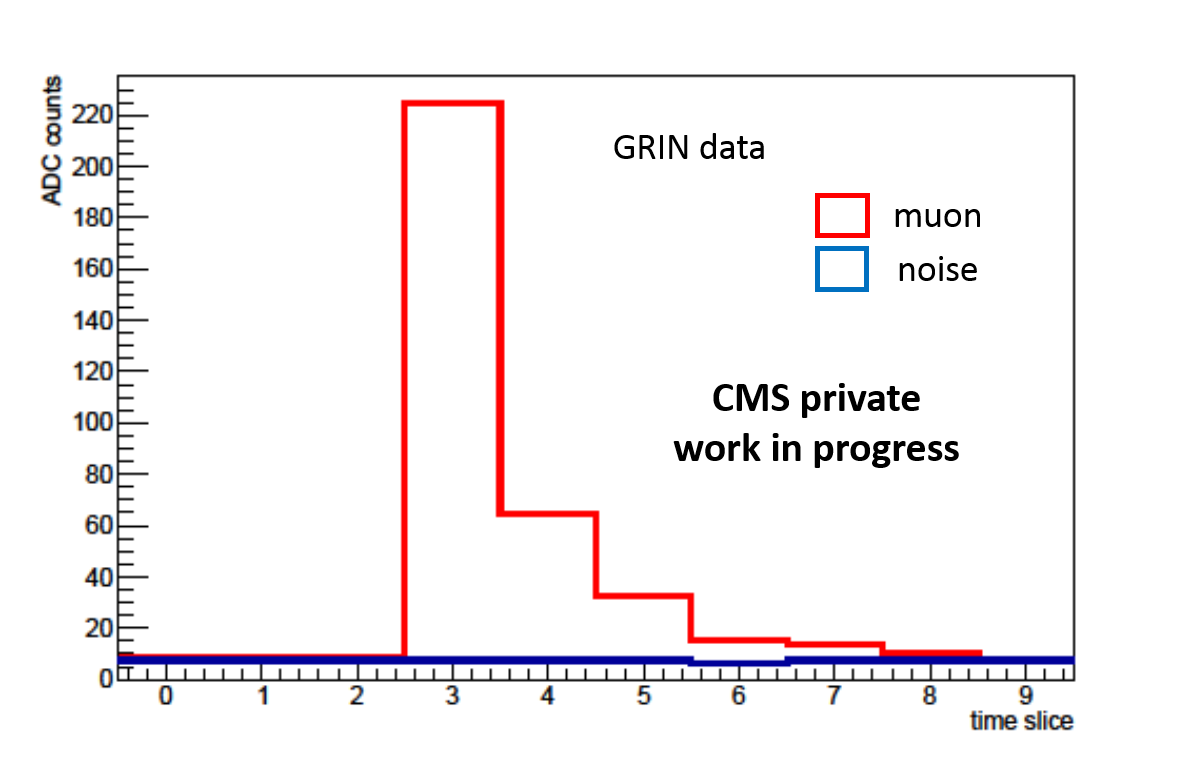
\includegraphics[width=0.70\textwidth]{Figures/erdogan/adc_vs_ts.png}
				\caption{The calibrated ADC counts versus the timeslices in which they are measured: In blue a tile is chosen, where interaction has occured (noise). In red is a tile with muon transition shown.}
				\label{fig:adc_vs_ts}
			\end{figure}
			In case of a muon transition the measured ADC counts in the corresponding timeslice are clearly higher than without muon transition.
			This means that seperating the muon signal from the noise is possible.
		\subsubsection{Purity studies}
			In \cite{dn2014-020} the funtionality of SiPMs is discussed.
			Studies on local HO data with so-called finger spectra are done and outlined in the section \ref{sec:hoSipmUpgrade}.
			Concerning the HO data from GRIN the signal in one randomly chosen HO tile is considered.
			In Fig.\ \ref{fig:noise_low} this signal distribution as a function of ADC counts is shown for an arbitrary tile.
			\begin{figure}[htbp]
				\centering
				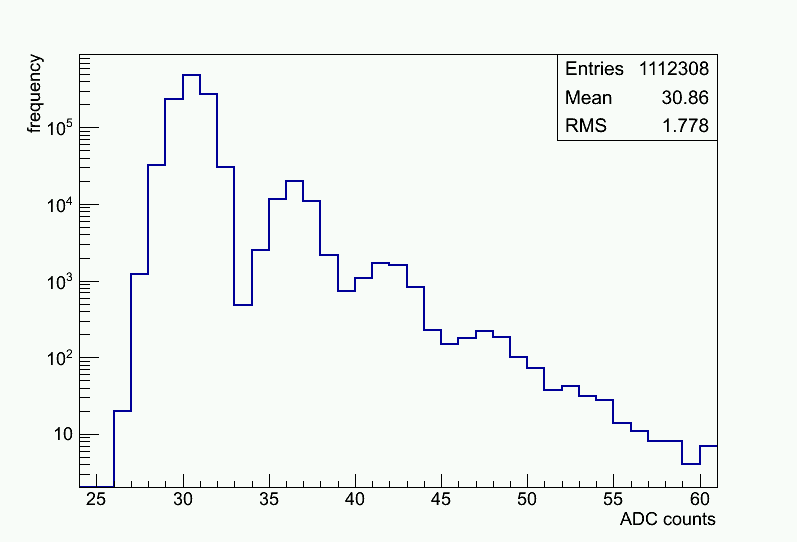
\includegraphics[width=0.70\textwidth]{Figures/erdogan/noise_low.png}
				\caption{The signal distribution as a function of ADC counts for a randomly chosen tile.}
				\label{fig:noise_low}
			\end{figure}
			The first peak at 32 ADC counts is the pedestal peak.
			Furthermore there are 3 additional peaks corresponding to up to 3 firing pixels of the SiPM.
			The distance between the peaks, which is the gain of the SiPM, is 6 ADC counts.
			All these observations are consistent with the expectations from the HO detector performance group as outlined in section \ref{sec:hoSipmUpgrade}.
			Since this study is done with only one tile per event the statistic is relatively low.
			To study the behaviour of the noise distribution with more data, all tiles per event without a muon transition should be taken into account.
			To do this first of all the tile where the muon went through has to be tagged.
			This is done by the \verb+TrackDetMatchInfo+ tool described in the previous subsection.
			Afterwards a safety region of 3x3 tiles around this tagged tile is defined.
			Now with all remaining tiles in all events the noise distribution can be determined (Fig.\ \ref{fig:noise_high}).
			\begin{figure}[htbp]
				\centering
				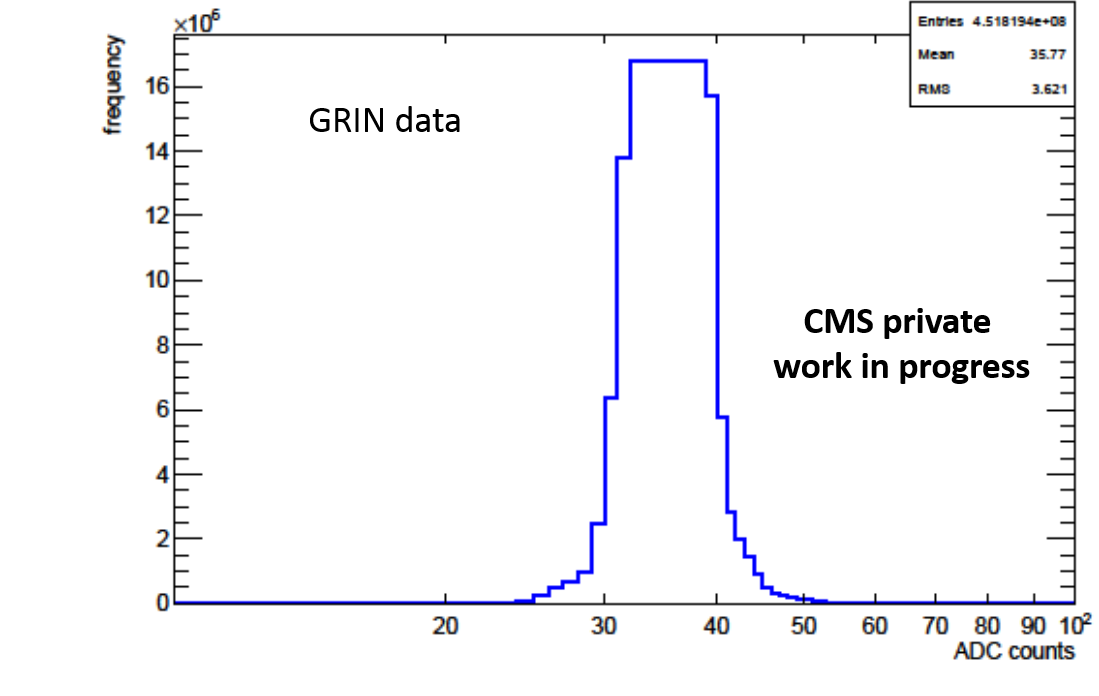
\includegraphics[width=0.70\textwidth]{Figures/erdogan/noise_high.png}
				\caption{The signal distribution as a function of ADC counts for all tiles without muon transition.}
				\label{fig:noise_high}
			\end{figure}
			The mean is at 36 ADC counts as expected and seen in the distribution with low statistic.
			However the fingers are not visible anymore.
			The reason for this is the smearing of the fingers due to statistical fluctuations.
			Furthermore the distribution drops steeply until in the higher bins there is no significant contribution anymore.
			Using this behaviour a purity $p$ of the muon signal can be defined:
			\begin{equation}
				p = \frac{\textnormal{number of entries below threshold}}{\textnormal{number of all entries}},
			\end{equation}
			thus above 60 ADC counts for instance it is not expected to have any noise contribution in the signal.
			In the section \ref{working_point} this value can be improved comparing the efficiency and the purity.
		\subsubsection{Efficiency studies}
			After having a method to estimate the purity the muon signal itself has to be analyzed.
			Using the \verb+TrackDetMatchInfo+ tool one can find the tiles where the muons are going through.
			Once the correct tiles are tagged, the DIGI information can be analyzed.
			For this purpose an integration over four timeslices is done to define the signal.
			The choice of the correct four timeslices is important and is done as described here:
			\begin{itemize}
			  \item Find the time slice $i$ with the highest ADC counts.
			  \item If $i$ is between the first and the seventh (inclusively) sum up ADC counts of the time slice $i-1$, $i+1$ and $i+2$ to the ADC counts of $i$.
			  \item Since this procedure is not working for $i=0$, $i=8$ or $i=9$ in these cases use time slices two to five for the integration.
			\end{itemize}
			In Fig.\ \ref{fig:efficiency1x1} the integrated value of ADC counts from tiles where a muon went through is plotted.
			\begin{figure}[htbp]
				\centering
				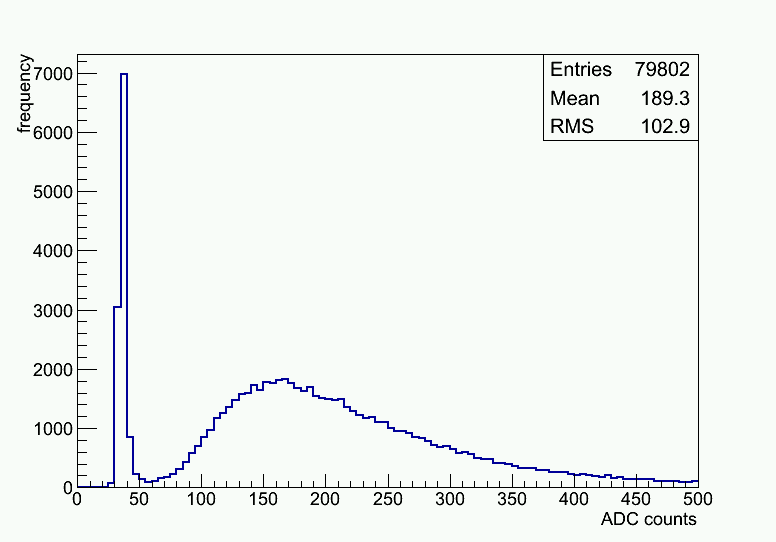
\includegraphics[width=0.70\textwidth]{Figures/erdogan/neighborhood1.png}
				\caption{The signal in ADC counts from tiles with muon transition}
				\label{fig:efficiency1x1}
			\end{figure}
			The main issue is the number of tiles with very low signals (first peak).
			Setting a threshold on the x axis, one can define an efficiency $\epsilon$
			\begin{equation}
				\epsilon = \frac{\textnormal{number of entries above threshold}}{\textnormal{number of all entries}},
			\end{equation}
			and the inefficiency $1-\epsilon$ respectively.
			If the threshold is set to 60 ADC counts, only 80\,\% of muons have a signal above threshold.
			The reason for this behaviour could be a first hint of detector inefficiencies.
			But also the functionality of the \verb+TrackDetMatchInfo+ tool can be doubted.
			To study the latter the search for the correct tile is not restricted to one tile predicted by \verb+TrackDetMatchInfo+ but all neighbor tiles are included.
			In this neighborhood the integration of timeslices is done as described above.
			The tile is chosen to be the correct tile if the value of the integrated ADC counts is maximum.
			In case of the matching tool being working correctly, the search in the neighbor tiles should have no effect on the signal distribution from Fig.\ \ref{fig:efficiency1x1}.
			\begin{figure}[htbp]
				\centering
				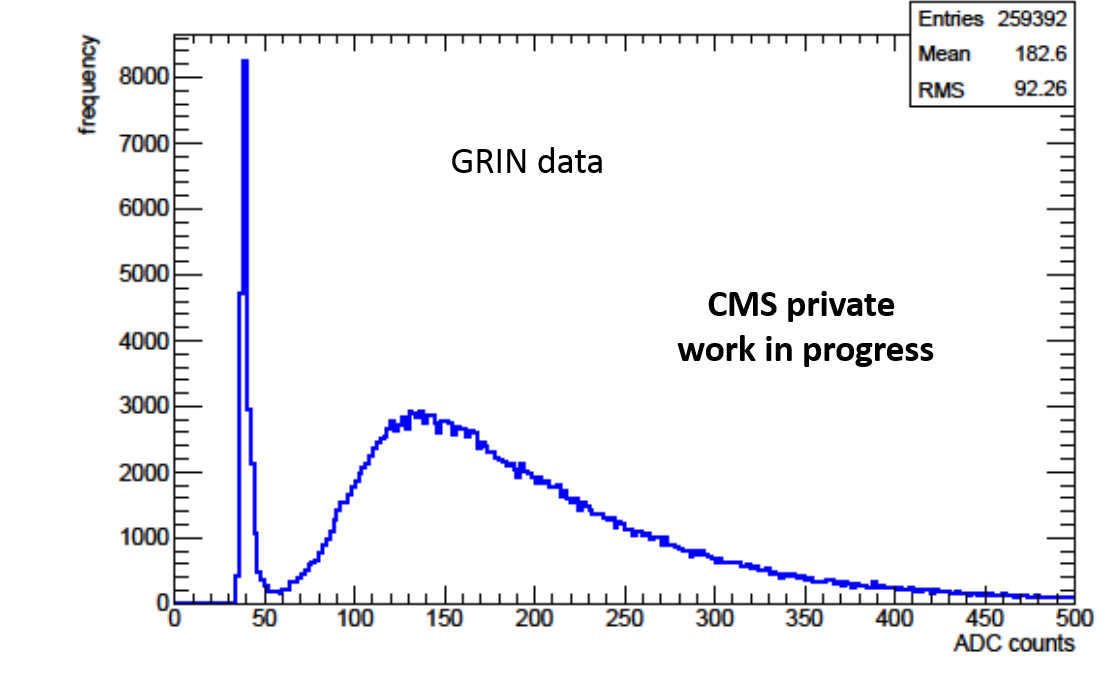
\includegraphics[width=0.45\textwidth]{Figures/erdogan/neighborhood2.png}
				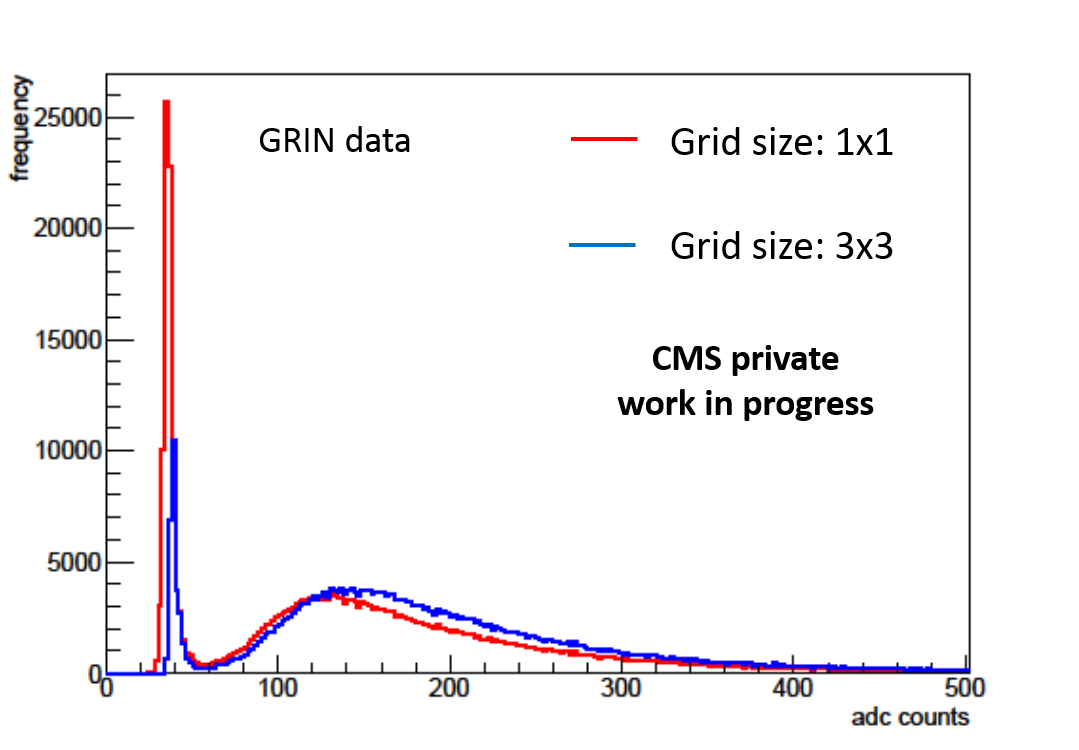
\includegraphics[width=0.45\textwidth]{Figures/erdogan/neighborhood.png}
				\caption{Left: Signal distribution in case of considering a 3x3 grid around the tile predicted by the matching tool. Right: Comparison between the left distribution (in blue) and the distribution from Fig.\ \ref{fig:efficiency1x1}}
				\label{fig:neighborhood}
			\end{figure}
			But in Fig.\ \ref{fig:neighborhood} one can see the improvement of the efficiency to around 92\,\% choosing a search area of 3x3 around the predicted tile.
			Increasing the size of this area to 7x7 has no significant effect on the distribution or efficiency.
			This means that the TrackDetMatchInfo is finding the correct tile in 80\,\% of all cases and in 12\,\% of all cases it misses it by one neighbor tile. \\
			The second issue is the shape of the signal.
			A Gauss convoluted Landau fit on the signal (above threshold) is shown in Fig.\ \ref{fig:langaus_bad}.
			\begin{figure}[htbp]
				\centering
				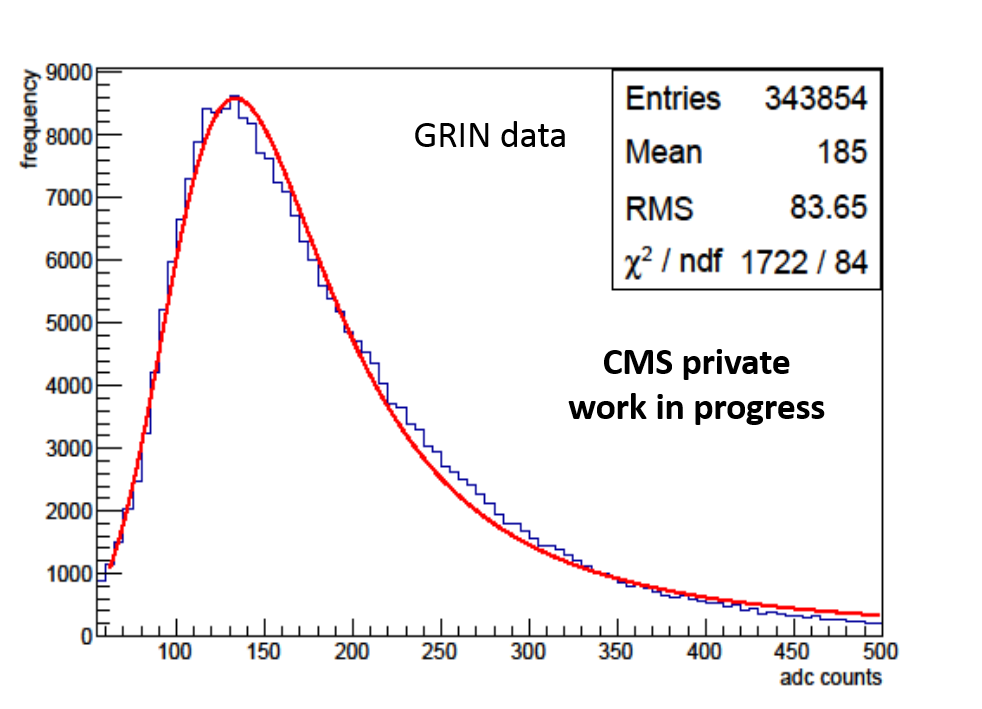
\includegraphics[width=0.70\textwidth]{Figures/erdogan/langaus_bad.png}
				\caption{The signal above a certain threshold from Fig.\ \ref{fig:efficiency1x1}. In red a Gauss convoluted Landau fit, which does not describe the behaviour very well.}
				\label{fig:langaus_bad}
			\end{figure}
			Obviously the shape can not be described with this fit.
			The reason is the difference in distances of tiles from the readout modules.
			The intensity of the light signals drops with the length of the fibre.
			Therefore one has to compare tiles with the same fiber lengths only.
			This is done in Fig.\ \ref{fig:langaus_good} resulting in a much better fit.
			\begin{figure}[htbp]
				\centering
				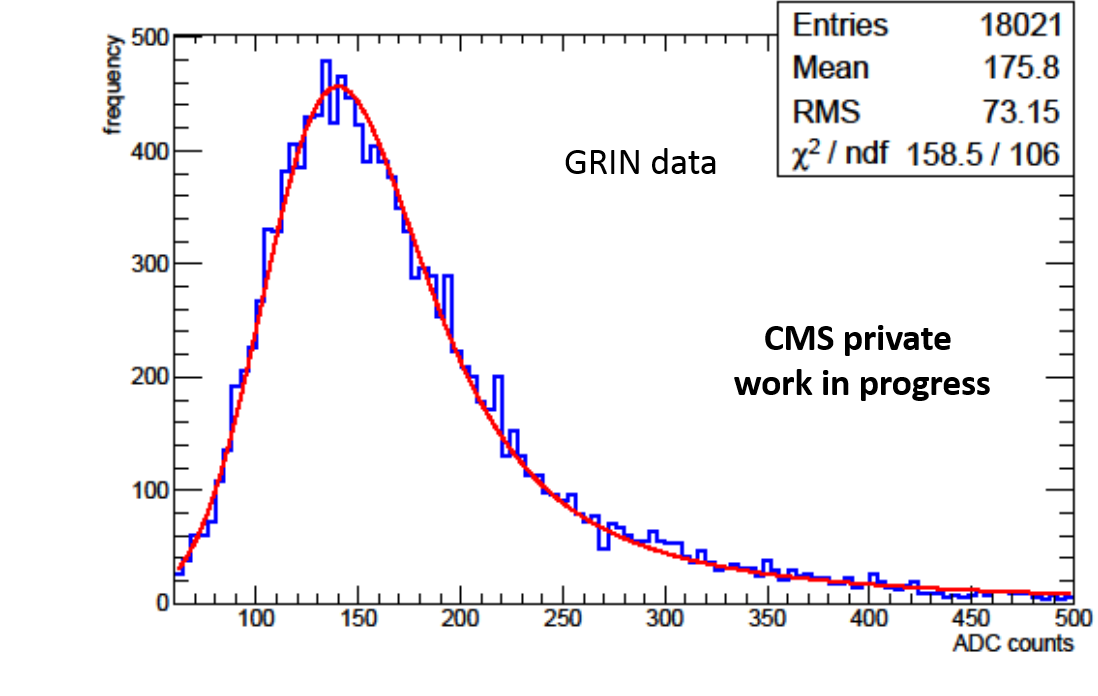
\includegraphics[width=0.70\textwidth]{Figures/erdogan/langaus_good.png}
				\caption{Signal distribution from tiles with muon transition, which can be compared due to their distance to the readout modules. In red again a gaus convoluted Landau fit with much better
				results.}
				\label{fig:langaus_good}
			\end{figure}
		\subsubsection{Working point for triggering muons}
		\label{working_point}
			The requirement for a good particle detector is working with high efficiency at high purity.
			In the previous sections we chose the thresholds for purity and efficiency arbitrarily by eye.
			After plotting those observables as a function of the threshold in ADC counts in the same histogram, we can define a more suitable threshold.
			In Fig.\ \ref{fig:pur_eff} this graph is depicted.
			\begin{figure}[htbp]
				\centering
				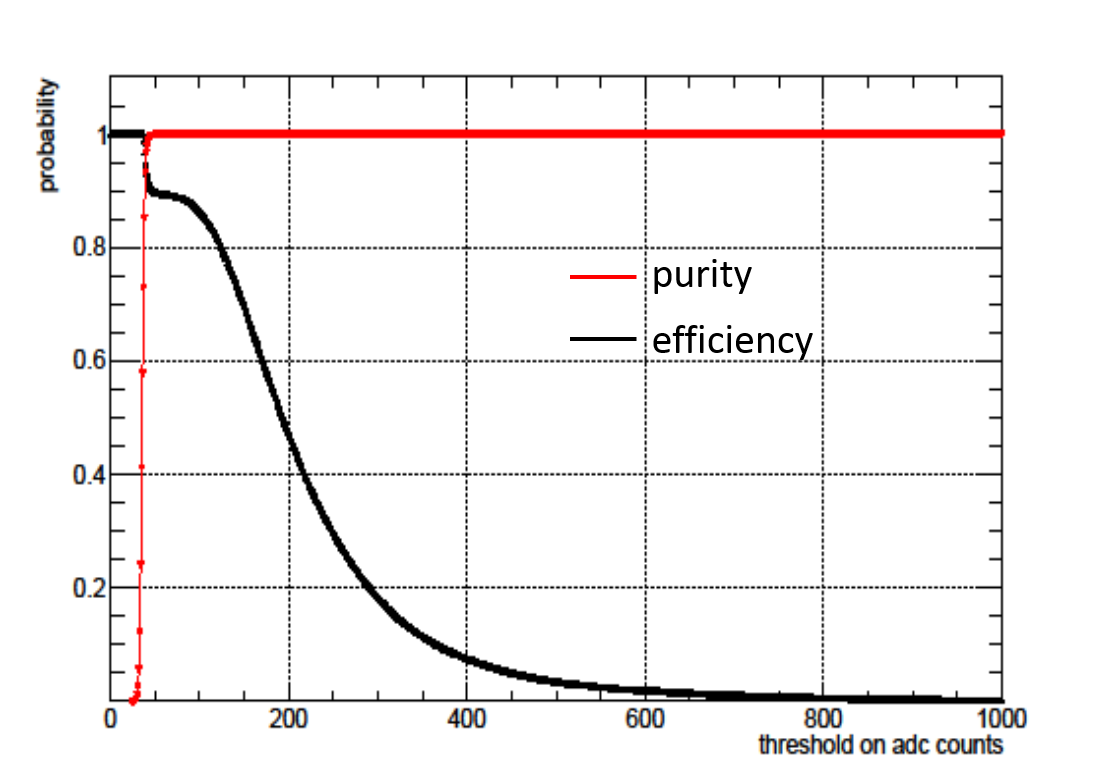
\includegraphics[width=0.45\textwidth]{Figures/erdogan/pur_eff.png}
				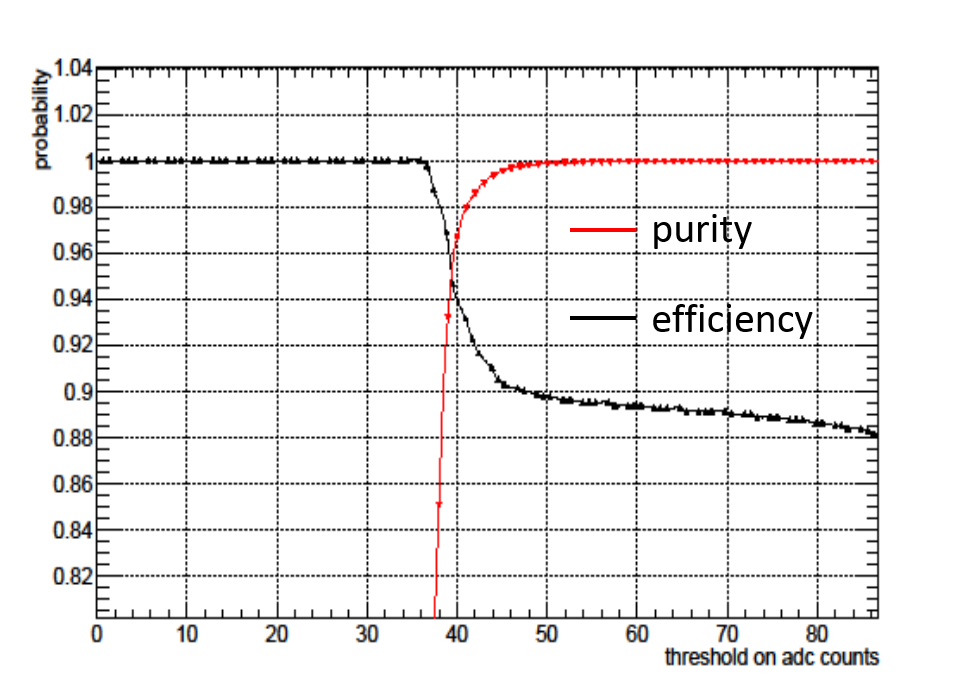
\includegraphics[width=0.45\textwidth]{Figures/erdogan/pur_eff_zoom.png}
				\caption{Left: Graph of purity and efficiency as a function of ADC counts. Right: Same graph zoomed in the intersection area.}
				\label{fig:pur_eff}
			\end{figure}
			The intersection point of both curves is at 39 ADC counts.
			At this point the purity accounts to 95\,\% and the efficiency to 95\,\%.
			In a more conservative way one can increase the threshold to 46 ADC counts leading to a highly pure signal of above 98\,\% by decreasing the efficiency to 90\,\%.
